
\begin{frame}
    \frametitle{Présentation}
    \begin{block}{Définitions}
	\begin{itemize}
	\item \textbf{Gestion de portefeuille :}
	      \begin{itemize}
	      \item Gérer des capitaux sous certaines contraintes
	      \item Choisir une stratégie d'investissement
	      \end{itemize}
	\item \textbf{Différents risques :}
	      \begin{itemize}
	      \item Financiers : marché, crédit, liquidité
	      \item Non financiers : modèle, perte extrême
	      \end{itemize}
	\item \textbf{Profils de rique :}
	      \begin{itemize}
	      \item Risk adverse
	      \item Risk neutral
	      \item Risk lovers/seekers
	      \end{itemize}
	\end{itemize}
    \end{block}


\end{frame}

\begin{frame}
    \frametitle{Actifs risqués}
	  \begin{figure}
	      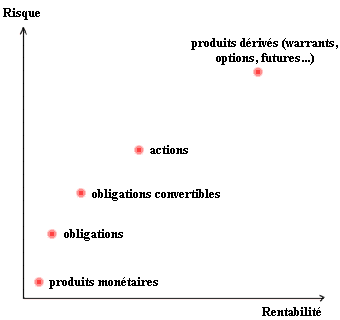
\includegraphics[scale=0.5]{images/actifsRisques.png}   
	  \end{figure}   
\end{frame}


\begin{frame}
    \frametitle{Diversification}
      \begin{figure}
	  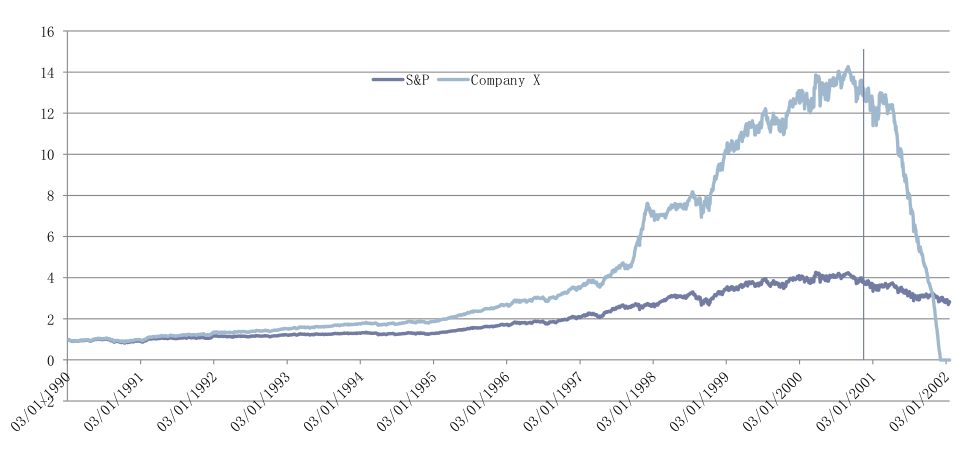
\includegraphics[scale=0.5]{images/exempleChuteEntreprise.png}   
      \end{figure}   
      \begin{block}{Intérêts}
	\begin{itemize}
	 \item Eviter les catastrophes
	 \item Réduire le risque
	\end{itemize}
      \end{block}

\end{frame}
